%=== CHAPTER TWO (2) ===
%=== Literature Review ===

\chapter{Literature Review}

\section{Visual SLAM}

\subsection{Introduction}
Simultaneous Localizaiton and Mapping (SLAM) is a technique for obtaining an unknown environment's 3D structure and sensor movement in the environment. Following years of development, SLAM-based application has become widespread, such as 3D modeling based on computer vision, self-driving cars and augmented reality(AR) visualization. 

In early SLAM algorithms, there exit many different modalities of sensors integrated in SLAM systems, such as rotary encoders, light detection and ranging radar (LiDAR), inertial sensors, GPS and cameras. In recent years, SLAM using cameras only,  specifically named as visual SLAM (vSLAM), has been actively discussed because of the simple, low-cost the sensor configuration, and  abundant information. But meanwhile this technique also brings more difficulties than others using integrated sensors\cite{taketomi2017visual}. 

vSLAM algorithms have proposed widely in the field of computer vision, robotics and AR. The low requirement on the modalities of sensors, requiring cameras only, is the major advantage of vSLAM technique, so that it is very suitable for low-cost unmanned vehicles, robots with limited load capacity and power supply like drones, or mobile devices such as camera-mounted tablets or smart phones.

However, the difficulties brought by vSLAM can not be ignored. Instead of obtaining depth and location information directly from LiDAR, GPS or depth camera in integrated SLAM systems, vSLAM technique needs to compute all these information from color or gray images, which reduces stability and accuracy for several estimation steps involved in this process. Also obviously the computational cost are significantly higher. Therefore, the problem of how to improve the performance and reduce computational cost of vSLAM has always been widely concerned.



%\subsection{Feature-based Algorithm}

%\subsection{Segmentation-based Algorithm}

\subsection{ORB-SLAM}
\label{chp:orbslam}
One of the state-of-the-art vSLAM solutions for single-robot systems is ORB-SLAM, initially proposed in \cite{mur2015orb}, and upgraded to a second version in \cite{mur2017orb}.

Initially proposed as a monocular SLAM system based on features, ORB-SLAM enables robots to map in real time small or large, indoor or outdoor environments with input of single camera images. The new vision has been upgraded to ORB-SLAM2 in \cite{mur2017orb} and can process monocular, stereo and RGB-D inputs. As stated in the proposed work \cite{mur2015orb}, ORB-SLAM is based on the main ideas of PTAM, the place recognition algorithm in \cite{galvez2012bags}, the use of covisibility information for large-scale operation \cite{strasdat2011double}, \cite{mei2010closing} and the scale-aware loop closure in \cite{strasdat2010scale}.  As a novel monocular SLAM system, the main contributions of ORB-SLAM are:
\begin{enumerate}[1.]
	\item In all tasks, the same features are used: tracking, mapping, closing of loops and relocation. Making the system more efficient, reliable and simple with the same features. And using ORB features enables GPU-free real-time performance, with signiticant invariance to changes in lighting and viewpoint. 
	\item In large environments, real-time performance. Due to the advantage of using a covisibility graph, the tracking and mapping modules are focused in a local visible area, independent of the global map. 
	\item Loop closing in real time. Optimizing a pose graph called the Essential Graph is adapted to perform the closing performance of the real-time loop. The Essential Graph is created from links to loop closures, strong edges in the covisibility graph, and a system maintained spanning tree. \item Real time camera relocation with exceptional viewpoint and illumination invariance. This improves the reuse of maps and also allows recovery from failure tracking. 
	\item A new robust and automatic initialization procedure 
	mode-selection-based that creates an initial map.
	\item A survival of the most appropriate approach to keyframe selection and map point, very restrictive in culling but generous in spawning. This policy enhances service life and improves the robustness of tracking because redundant key frames are discarded.
\end{enumerate}

ORB-SLAM system, see on Figure \ref{fig:orbslamoverview}, performs three threads that run in parallel: tracking, local mapping and loop closing. 

%The tracking thread is in charge of localizing the camera with every frame and deciding when to insert a new keyframe.	The module firstly match current frames with previous frames, and optimize the pose using motion-only bundle adjustment. If the 

\begin{figure}[H]
	\centering
	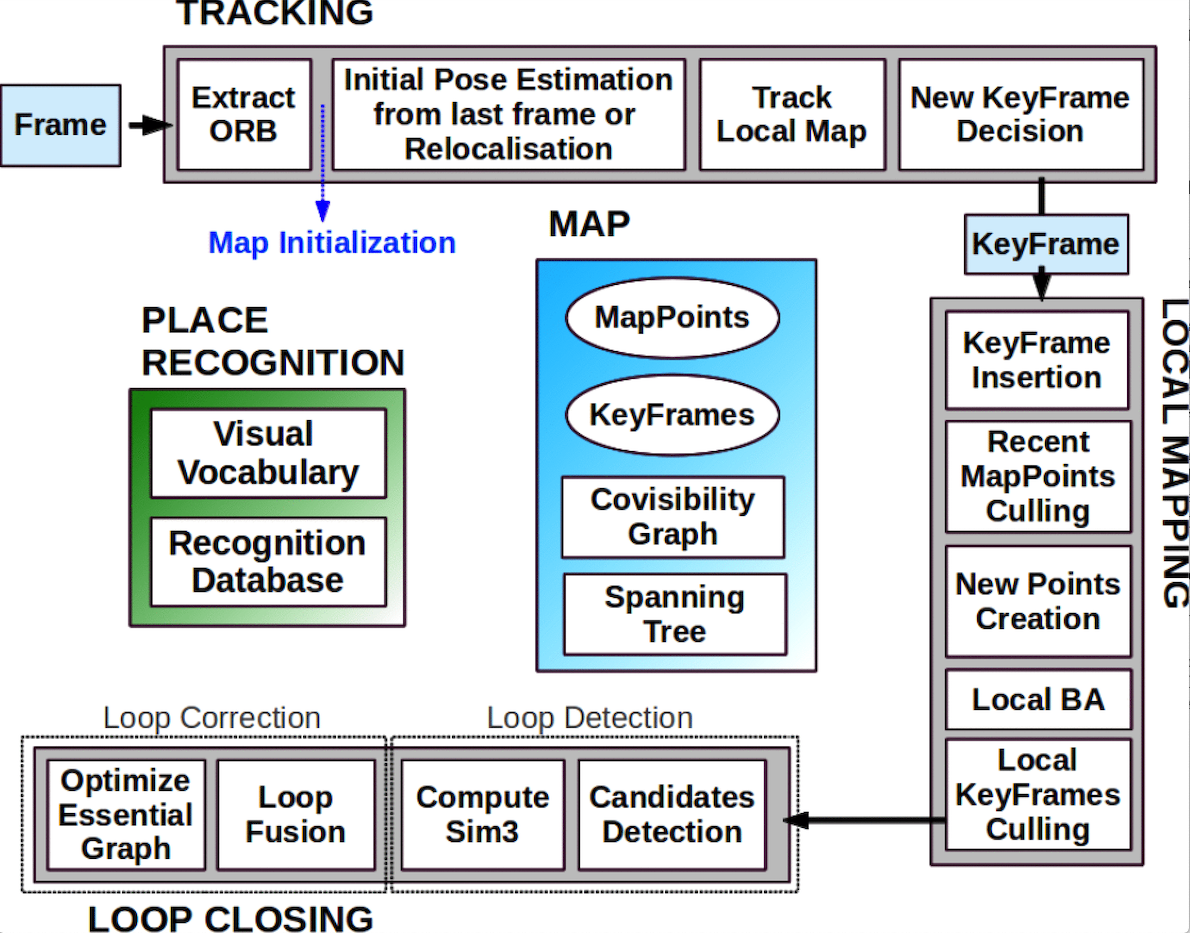
\includegraphics[width=5in]{Chapter2/ORBSLAMOverview.eps}
	\caption{ORB-SLAM system overview.}
	\label{fig:orbslamoverview} 
\end{figure}

\section{Multi-robot SLAM}

Multi-robot SLAM (MR-SLAM) uses several collaborative robots to map an unknown environment as an extended system of single-robot SLAM. However, the extension can not be easily implemented as each client maps their surroundings on their own local frame of reference. Therefore, in order to merge the sub map of several clients into a consistent global map, the map fusion server needs to be able to connect and find the transformation between different local client reference frames.The environment can be mapped significantly faster using MR-SLAM technique on a cluster of multi ground or hybrid robots and the uncertainty in the system can be reduced due to data redundancy.
Furthermore, if separate robots are equipped with heterogeneous sensors, the fused global map may contain much more feature information than a single robot map. Another obvious advantage is the robustness of one or more robots to fail, particularly when data is decentralized. 

As concluded in \cite{10.1007/978-3-319-78452-6_15}, besides the advantages above, MR-SLAM systems also face problems and choices in the following aspects:

\begin{inparaenum}[1.]
	\item Centralization or Decentralization. Determining where data processing takes place is one of the main questions building MR-SLAM systems. Data is processed in centralized approaches on a central server, performing the task to fuse  the information collected by all robots and distribut global map information to clients to improve their ability to self-locate\cite{forster2013collaborative, li2012laser,li2017corb}. By contrast, decentralized MR-SLAM systems usually have several clients, interconnected with each other and managed by a coordinating structure that allows systems to efficiently deal with large numbers of agents\cite{bresson2013consistent,fox2006distributed}. 
	
	\item Communication and information sharing. Decentralized data processing and consistent global map sharing have high requirements for communication bandwidth, latency and coverage area. Not only the connection characteristics e.g. connection architecture and protocol, but also the transmitting period and content etc. need to be selected carefully when designing MR-SLAM software systems.
\end{inparaenum}

\subsection{CORB-SLAM}
Proposed by F.Li et al. in \cite{li2017corb}, CORB-SLAM is centralized visual MR-SLAM systems based on ORB-SLAM2. As presented in Figure \ref{fig:corbslamoverview}, the system of CORB-SLAM consists of robot-end clients running ORB-SLAM2 modified to transmit map information via ROS and a central server responsible to fuse maps and resend global maps.
\begin{figure}[H]
	\centering
	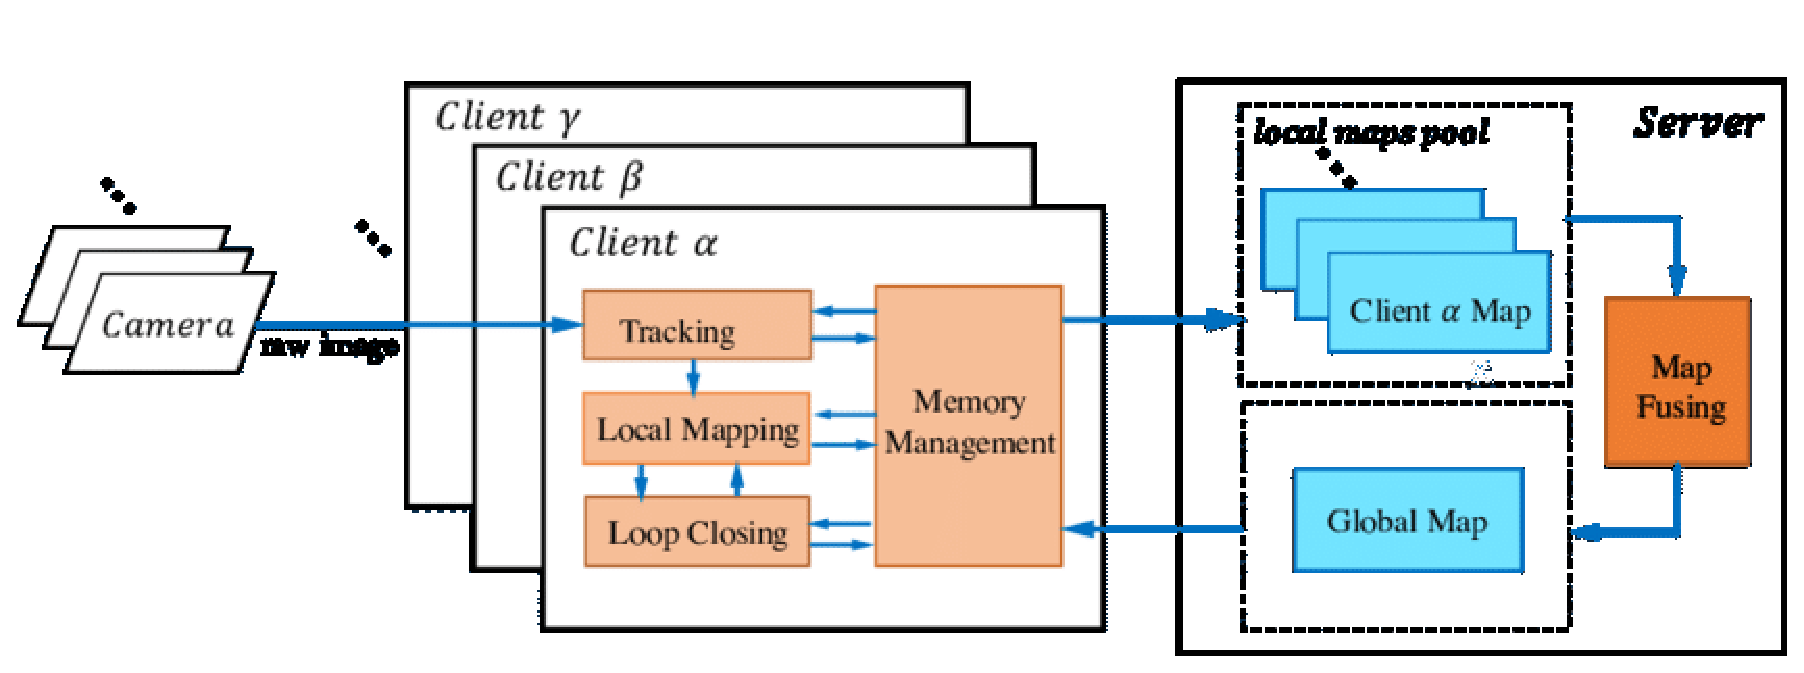
\includegraphics[width=5in]{Chapter2/CORBSLAMOverview.eps}
	\caption{The structure of CORB-SLAM system.}
	\label{fig:corbslamoverview} 
\end{figure}

\subsubsection{CORB-SLAM Client}
The robot-end client of CORB-SLAM is an ORB-SLAM client extended to have the functionality to communicate with the server, transmitting the local map information, with all functions and modules in original ORB-SLAM as listed in Chapter \ref{chp:orbslam} reserved.

\begin{figure}[H]
	\centering
	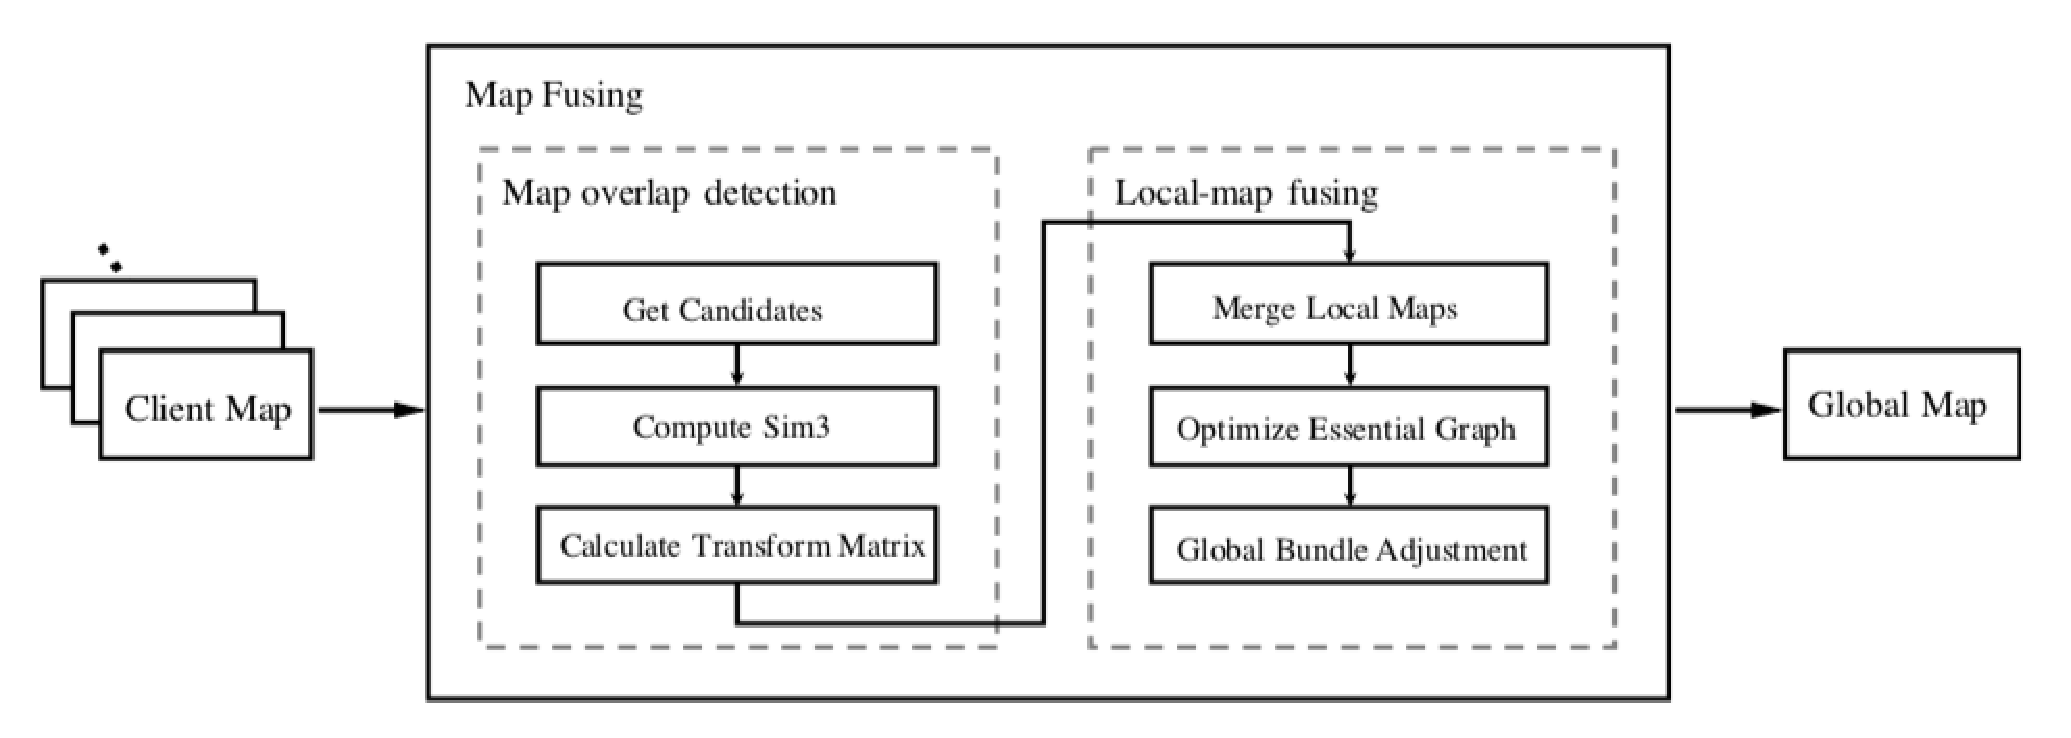
\includegraphics[width=5in]{Chapter2/corbslamserver.eps}
	\caption{The flowchart of Map Fusing module.}
	\label{fig:corbslamserver} 
\end{figure}

\subsubsection{Map Fusion}
The server's map fusion module receives and fuses the clients ' local maps to achieve an optimized global map. Figure \ref{fig:corbslamserver} shows the map fusion algorithm, which includes three main parts: global map initialization, map overlap detection, and local map fusion.

\begin{enumerate}[1.]
	\item Initializing global map
	
	As the server system starts at the beginning, the initial global map is set to empty. As clients keep mapping and creating their local maps, the server receive data of local maps. After a first local map reaches the server, it will set as the initial global, based on which the global reference frame is decided.
	
	\item Map overlap detection
	
	To calculate relations between local maps, the server firstly detects the overlaps among local maps and then computes the transform matrices using Perspective-n-Point method.
	
	The map overlap detection module follows the same solution of ORB-SLAM2, which firstly extract keypoints from input images using ORB features, then compute similarities between images by distance between image descriptors based on Bag of Binary Words (DBoW3) approach.
	Then, after map overlaps are detected, RANSAC iterations are adopted to calculate the 7 degrees-of-freedom (DoF) transform matrix between the current keyframe and all rough candidates detected. With enough inliers, a similar candidata, $K_{\alpha}$ is optimized. If an enough number of inliers are calculated, the overlap with $K_\alpha$ is accepted with the pose of $K_\alpha$, $T_{wc}$ calculate at the same time during optimization.
	
	\item Local-map fusing 
	
	Local maps are merged into the consistent global map after an acceptable transform matrix has been obtained. Using Bundle Adjustment (BA), a global 7 DoF optimization is then performed to suppress map errors caused by various SLAM clients.
\end{enumerate}

After all process finished, the fused global map is resent to clients, and each client continues its own work to detect loop closure and correct loops on the received global map. If the global map is updated by computation on clients, the changes will be uploaded to server to update the map, and further transmitted to other clients by the server.

\section{Illumination Variance}

\subsection{Appearance Change From Illumination}

Facing appearance changes is an ongoing challenge for vision systems concerned with locating in known environments. Changes in appearance can result from several sources, for example, \begin{inparaenum}[(i)]
	\item different lighting conditions,	
	\label{ls:appearancechange1}
	\item varying weather conditions, and
	\label{ls:appearancechange2}
	\item dynamic objects such as pedestrians or vehicles.
	\label{ls:appearancechange3}
\end{inparaenum}

In previous work by Colin McManus et al., they showed how to leverage knowledge of previous 3D structure to suppress distracting objects for improved pose estimation in busy urban environments \cite{mcmanus2013distraction}, and how to cope with long-term variation in appearance caused by changing weather conditions\cite{churchill2012practice}. They proposed a new approach to addressing problem in \cite{maddern2014illumination} called the Illumination Variance Approach. 

Appearance change caused by different lighting conditions in (\ref{ls:appearancechange1}) is illustrated in Figure \ref{fig:shadecompare1} with pictures selected from St Lucia dataset \cite{glover2010fab}. Compared to approaches proposed in \cite{mcmanus2013distraction} and \cite{churchill2012practice}, illumination variance approach is not model-based, requiring less computational cost. And in most of applications of vSLAM, appearance changes caused by (\ref{ls:appearancechange1}) are a more common problem than (\ref{ls:appearancechange2}, \ref{ls:appearancechange3}). Therefore, how to combine illumination variance approach with multi-robot SLAM algorithms, to improve the performance of place recognition modules in environments under changing illumination conditions, is one of the major objectives focused on in this work.

\begin{figure}
	\centering
	\subfigure[pic1.]{
		\begin{minipage}[t]{0.4\linewidth}
			\centering
			\includegraphics[width=2in]{Chapter2/shadecompare1-0.eps}
			%\caption{fig1}
		\end{minipage}
	}
	\subfigure[pic2.]{
		\begin{minipage}[t]{0.4\linewidth}
			\centering
			\includegraphics[width=2in]{Chapter2/shadecompare1-1.eps}
			%\caption{fig2}
		\end{minipage}
	}
	\caption{Appearance changes caused by different lighting conditions. Pictures are selected from St Lucia dataset recording on 10/09/2009 8:45 am and 2:10 pm}
	\label{fig:shadecompare1}
\end{figure}

\subsection{Formulation}
Illumination variance approach proposed in \cite{maddern2014illumination}, is a simple method based on only one equation computing illumination variant images. The basic idea of this approach is to map color images to an illumination invariant color space, where illumination change caused by different lighting condition like shade can be suppressed. The mapping equation
is presented in Equation \ref{eq:iifinal}.

\begin{equation}
I=\log(R)-\alpha\log(G)-(1-\alpha)\log(B)
\label{eq:iifinal}
\end{equation}

Where, $R, G, B$ are the raw image color channels and $I$ is the resulting invariant image illumination. As shown in \ref{eq: ii1}, $\alpha$ is a parameter that depends on each color channel's peak spectral responses ($ \lambda R, \lambda G, \lambda B$), normally available in camera specifications. 

\begin{equation}
\frac{1}{\lambda_R}=\frac{\alpha}{\lambda_G}+\frac{1-\alpha}{\lambda_B}
\label{eq:ii1}
\end{equation}

Therefore, considering the peak spectral responses, $\alpha$ can be easily calculated as exposed in Equation \ref{eq:ii2}.

\begin{equation}
\alpha=\frac{(\frac{\lambda_B}{\lambda_G}-\frac{\lambda_B}{\lambda_R})}{(1-\frac{\lambda_B}{\lambda_R})}
\label{eq:ii2}
\end{equation}

the result images of illumination variance conversion are showed in Figure \ref{fig:iicompare1}.

\begin{figure}
	\centering
	\subfigure[pic1.]{
		\begin{minipage}[t]{0.4\linewidth}
			\centering
			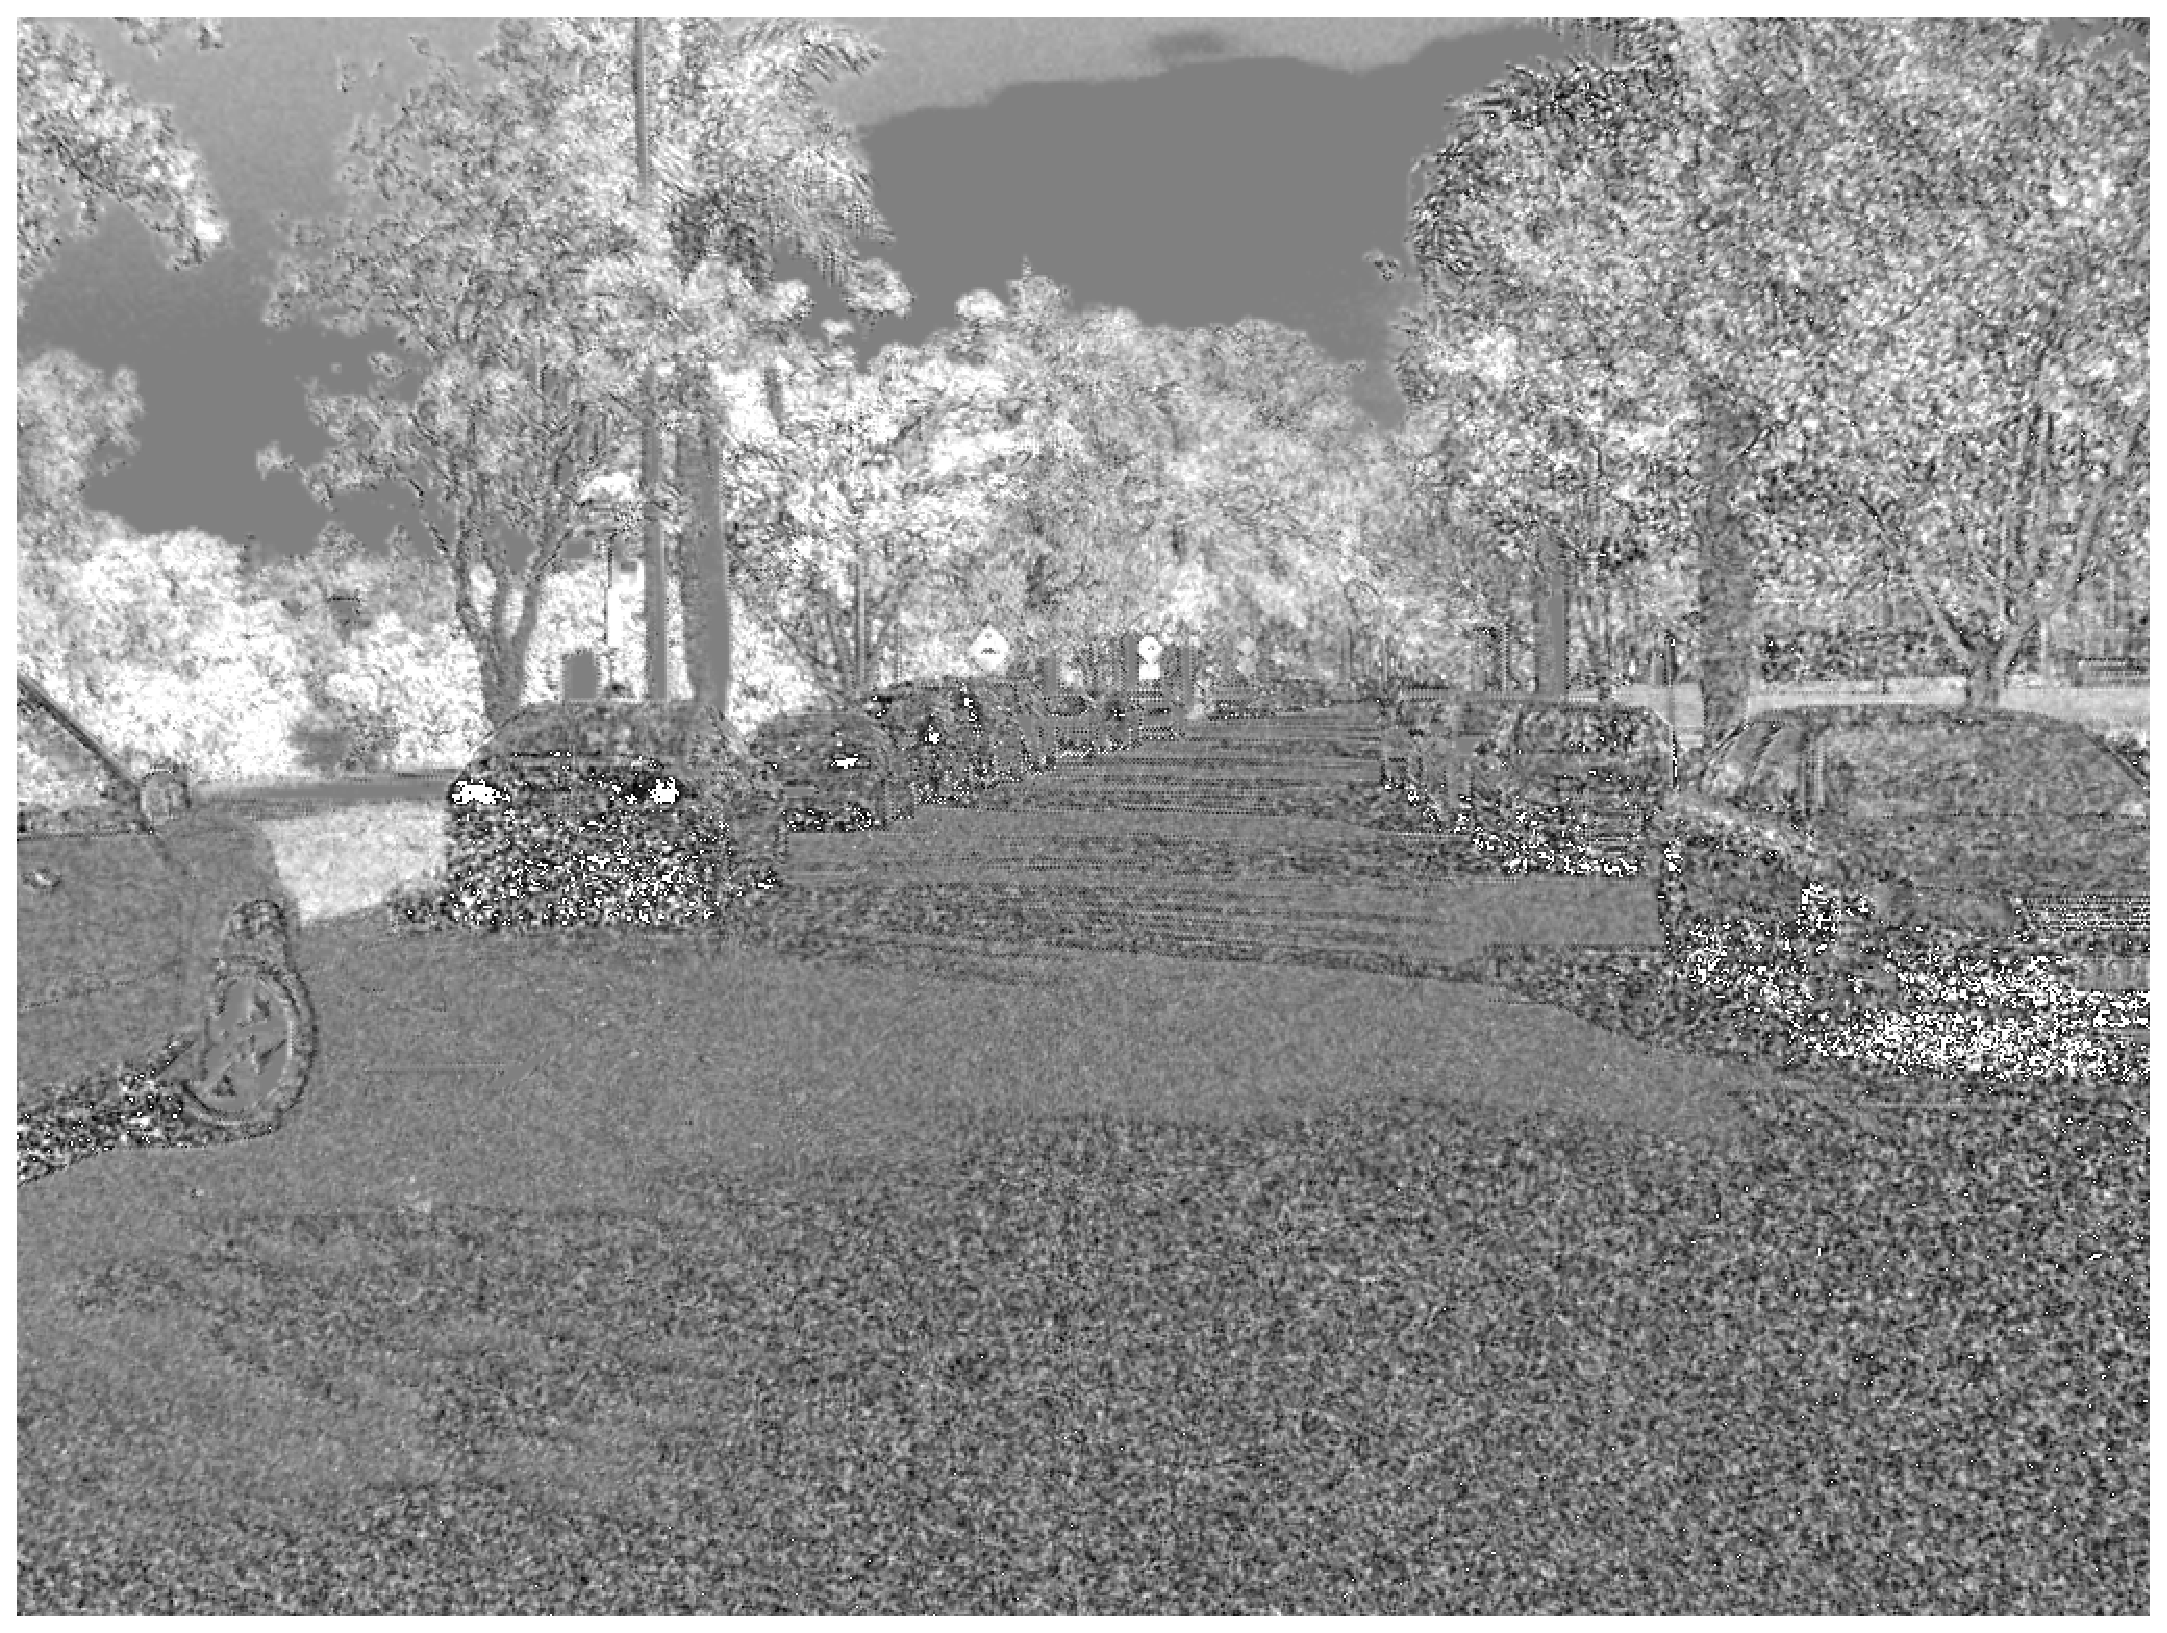
\includegraphics[width=2in]{Chapter2/iicompare1-0.eps}
			%\caption{fig1}
		\end{minipage}
	}
	\subfigure[pic2.]{
		\begin{minipage}[t]{0.4\linewidth}
			\centering
			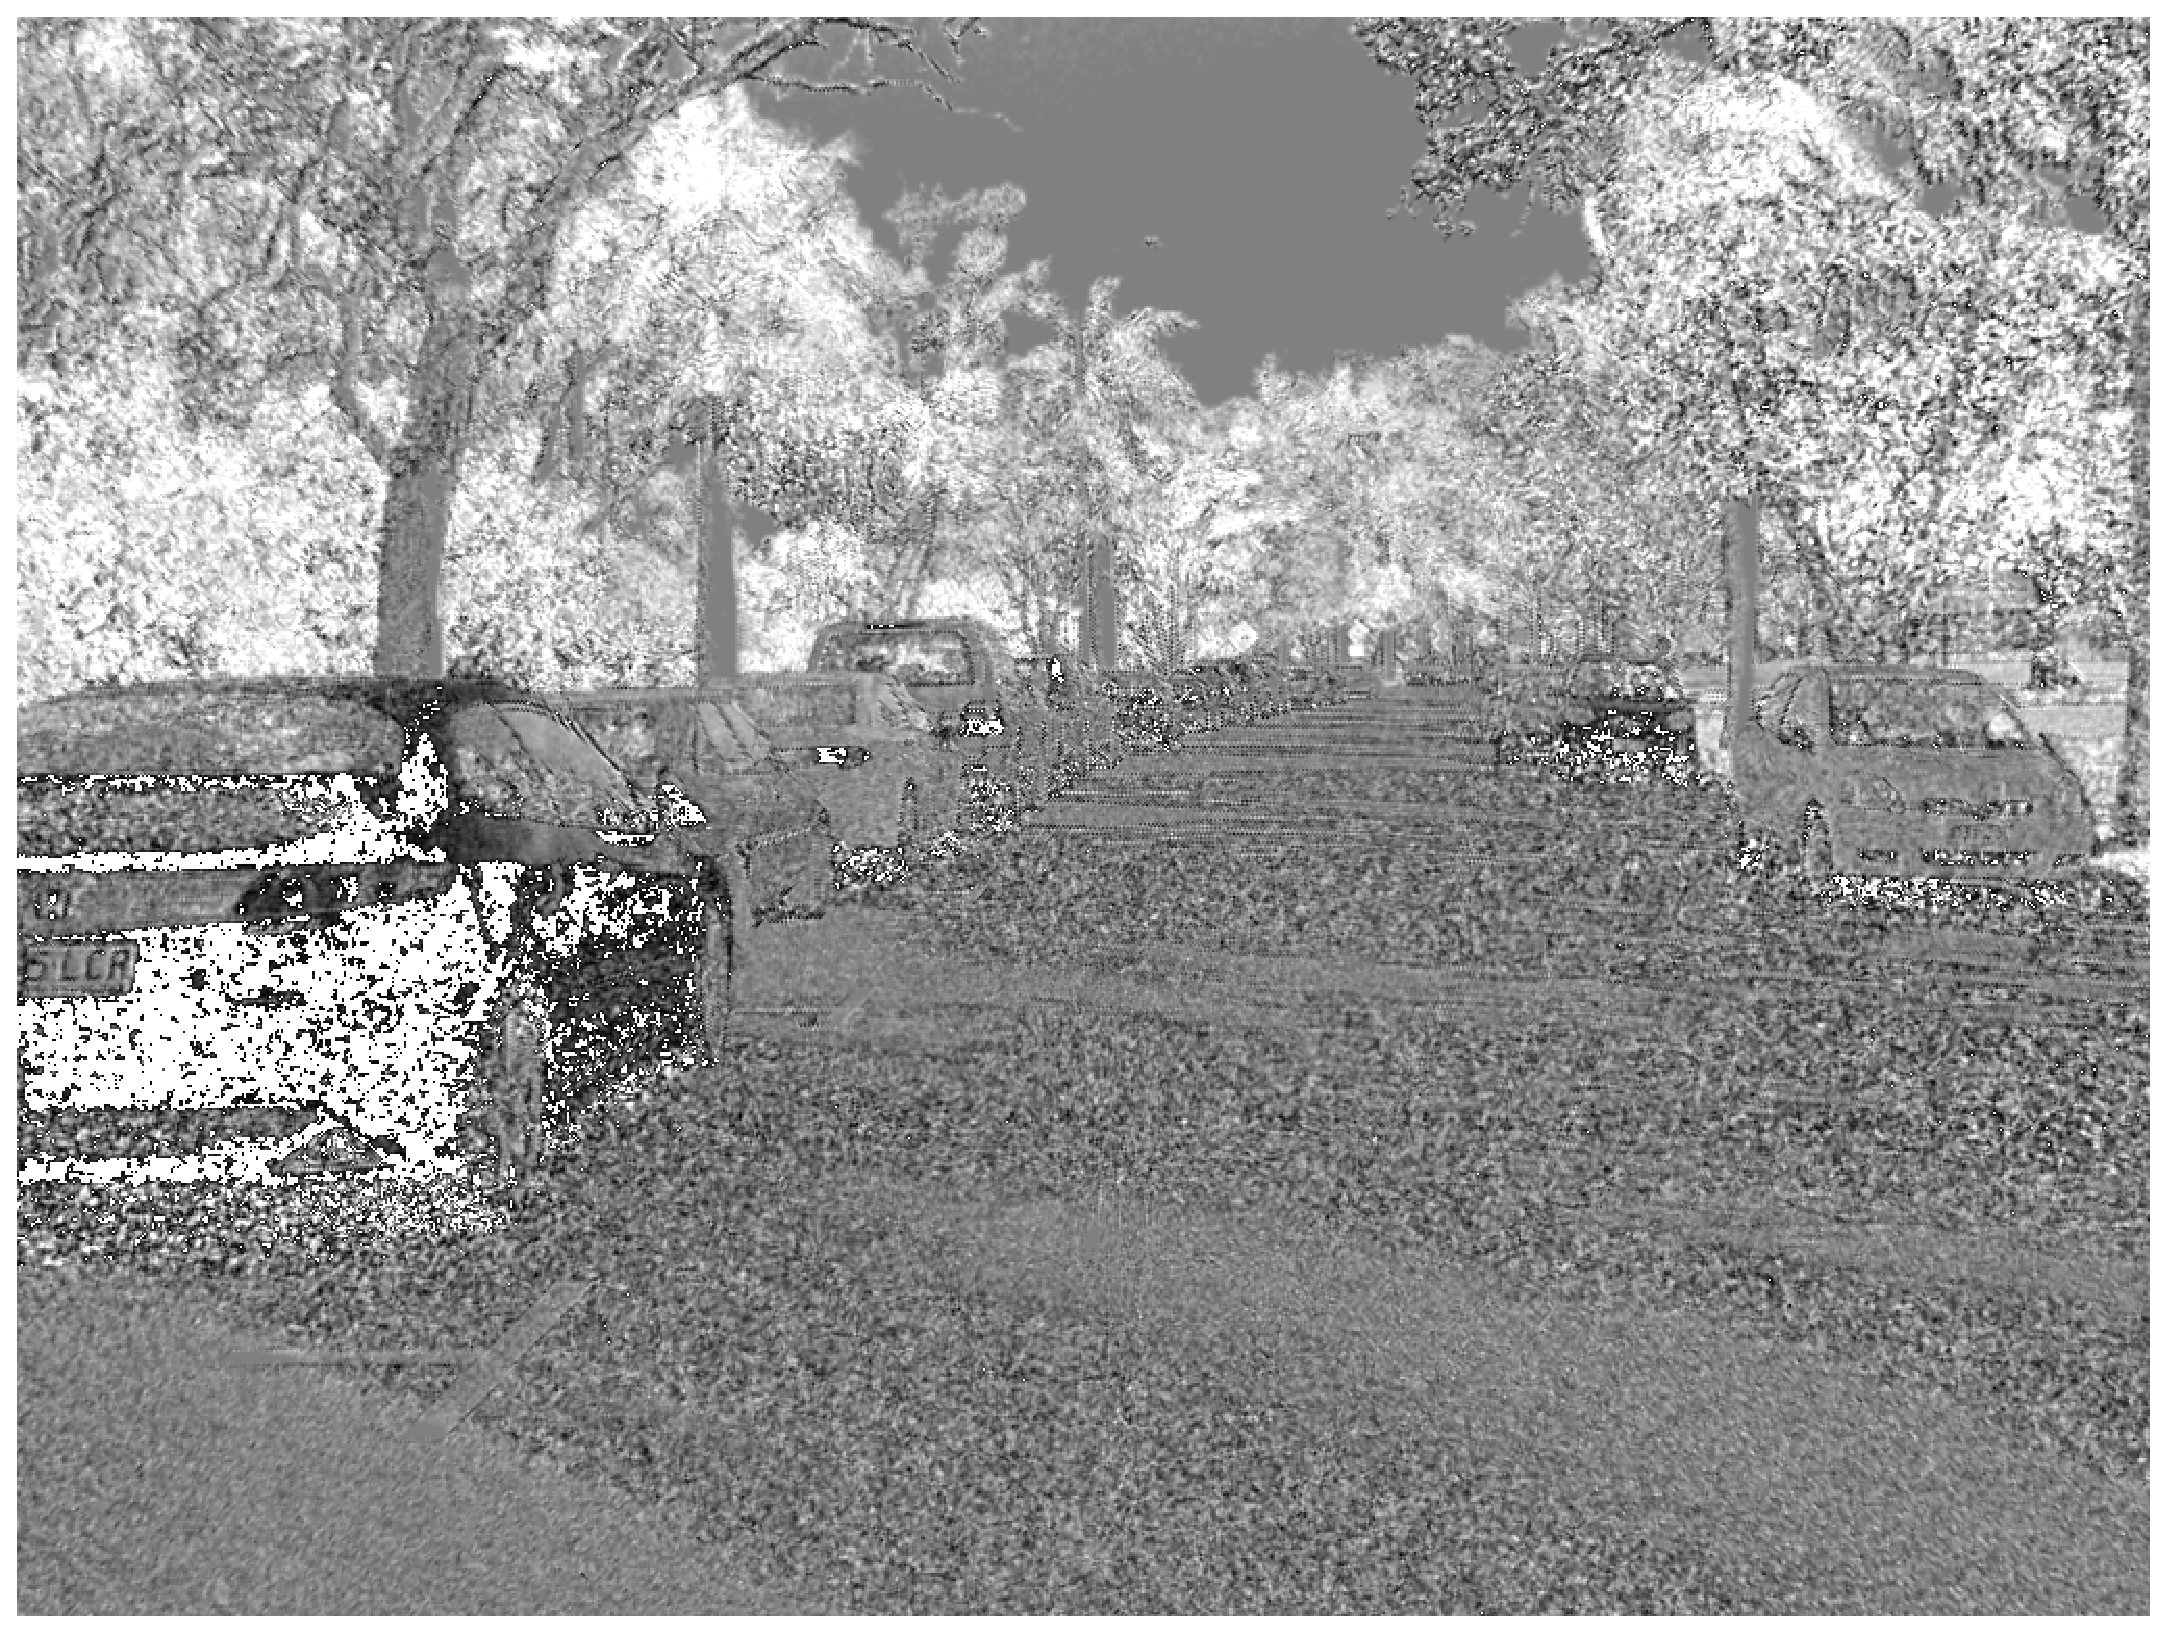
\includegraphics[width=2in]{Chapter2/iicompare1-1.eps}
			%\caption{fig2}
		\end{minipage}
	}
	\caption{Illumination invariance result images in St Lucia dataset. It shows how this approach suppress the effects caused by sun}
	\label{fig:iicompare1}
\end{figure}

\subsection{Application of Localization}
An open source toolbox called OpenABLE is implemented in \cite{arroyo2016openable} for lifelong visual localization. The proposed implementation in \cite{arroyo2016openable} uses the philosophy of the topological location recognition approach called ABLE introduced in \cite{arroyo2014bidirectional, arroyo2014fast, arroyo2015towards} using illumination variant images for relocation. 

A graphic representation about how the methodology proposed by OpenABLE is showed in Figure \ref{fig:openableoverview}.

\begin{figure}[H]
	\centering
	\includegraphics[width=5in]{Chapter2/OPENABLEOverview.eps}
	\caption{A graphic demonstration about how ABLE works.}
	\label{fig:openableoverview} 
\end{figure}

The limitation of illumination variance approach is the transformation process produces resultant images with low resolution because all pixel values are turned into log values. These low-resolution resultant images still can be used as the input images of visual topological localization where high resolution images are actually not needed. But in the mapping task, illumination variant images are too blurry to estimate camera motion and then reconstruct the map. Therefore, to improve the mapping performance in changing illumination conditions, rgb images and illumination variant images are both needed to perform relocalization and mapping, as the block-flow proposed in \cite{mcmanus2014shady} presented in \ref{fig:iioverview}.

\begin{figure}[H]
	\centering
	\includegraphics[width=5in]{Chapter2/COISLAMOverview.eps}
	\caption{Block-flow diagram of the combined stereo localisation approach.}
	\label{fig:iioverview} 
\end{figure}

In the framework presented in \ref{fig:iicompare1}, there is a second localizer making use of illumination invariant images in parallel with the main localization system. In \cite{maddern2014illumination}, although the metric relative poses calculated from illumination variant images tends wo be more noisy, the integrated localizer are less likely to fail if the scene appearance change is due to sunlight intensity direction or spectrum variation.

%=== END OF CHAPTER TWO ===
\newpage
